\chapter{Calculus: There's Sum Difference}\label{apx:calculus}

Calculus is one of the most useful set of mathematical techniques that a
geophysicist employs in their toolkit.  While some physics derivations can be
done with algebra, they are often far simpler to express and perform in terms of
calculus.  While many students place a mental barrier at the mere mention of
calculus, many of the concepts are really quite simple.

\section{Derivatives: How fast am I going?} \label{apx:derivatives}

\subsection{Rates of change}
Something you are undoubtably familiar with is traveling.  Traveling from home
to school in a car, on a bus, by foot?  In my case I biked to uni this morning.
I started at home (let's call it point $H$) at $t_0$ and arrived at the uni
(point $U$) some time later, $t_1$, for a total travel time $\Delta t = t_1 -
t_0$.  The distance traveled as the crow flies---there are no crows here... as
the magpie(?) flies---going from $H$ to $U$ is $\Delta x = x_1 - x_0$.

\vspace{8pt}
\noindent {\it How fast was I travelling?}

We can write my speed as
\begin{align*}
    \mathrm{speed} = & \frac{\mathrm{distance travelled}}{\mathrm{time elapsed}} \\
    v = & \frac{\Delta x}{\Delta t} .
\end{align*}
Graphically this represents the {\it slope} of a line on our graph
(Figure~\ref{fig:vavg1}).
\begin{figure}[hbt]
    \centering
    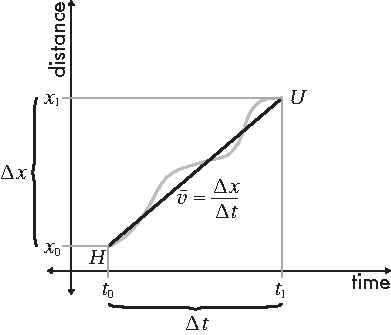
\includegraphics[]{math_primer/figures/average_velocity.pdf}
    \caption{Average velocity on the bike ride beween home and work.}
    \label{fig:vavg1}
\end{figure}

But of course I didn't travel at a constant rate.  The speed we just expressed
was the average speed,
\begin{equation*}
    \bar{v} = \frac{\Delta x}{\Delta t} .
\end{equation*}
So lets redraw the time-distance curve to something more realistic
(Figure~\ref{fig:vavg2}).
\begin{figure}[hbt]
    \centering
    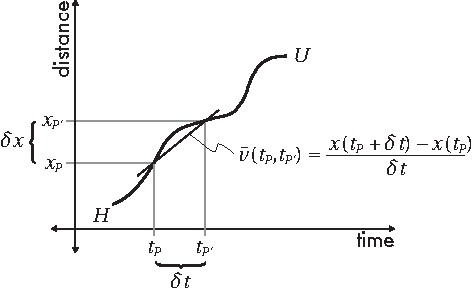
\includegraphics[]{math_primer/figures/average_velocity2.pdf}
    \caption{Average velocity during a short interval of time.}
    \label{fig:vavg2}
\end{figure}

\vspace{8pt}
\noindent {\it What was my speed as a function of time, i.e. v(t)?}

To derive this let's look first at how fast was I traveling at a single point,
$P$.  As we shown above, the speed is the slope of a line.  But we have a curve.
So lets take another point, $P'$, some time after $P$.  I passed $x_P$ at $t_P$
and $x_{P'}$ at $t_{P'}$.  We can compute the {\it average} speed between these
two points in time as
\begin{equation*}
    \bar{v}(t_P,t_{P'}) = \frac{x_{P'} - x_P}{t_{P'} - t_P} 
        = \frac{\delta x}{\delta t}.
\end{equation*}
But as before let's call the interval in time $\delta t$, which is $\delta t =
t_P - t_{P'}$.  And since $x$ is a function of time, $x = x(t)$.  So lets
rewrite the previous equation
\begin{equation*}
    \bar{v}(t_P,t_{P'}) = \frac{x(t_P + \delta t) - x(t_P)}{\delta t} .
\end{equation*}
``Ah,'' you say, ``but this is still an average velocity, we still don't know
the velocity at P.''  So what if we move the point $P'$ closer to $P$ and closer
still and then even closer until the two points $P$ and $P'$ are almost
coincident, i.e. $\delta t$ approaches 0 (Figure~\ref{fig:vinst}).
\begin{figure}[hbt]
    \centering
    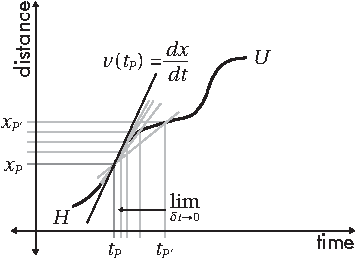
\includegraphics[]{math_primer/figures/instantaneous_velocity.pdf}
    \caption{Approximation of the instantaneous velocity by computing the
    average over smaller and smaller time intervals.}
    \label{fig:vinst}
\end{figure}
It is still an average, but the average will---assuming the function is {\it
continuous} and well-behaved---become a more accurate estimate of the {\it
instantaneous} speed at $t_P$.  We call the process of moving $P'$ towards $P$
as a {\it limit}, which we write as
\begin{equation*}
    \lim_{\delta t \to 0} \frac{x(t_P + \delta t_P) - x(t_P)}{\delta t} ,
\end{equation*}
In words we would say the ``in the limit $\delta t$ approaches 0...''  If our
assumptions hold true, then we are computing the average speed on a time
interval so small that it is effectively equal to the instantaneous speed at
$t_P$.  So we will now write this result not as the average but as the
instantaneous speed,
\begin{equation*}
    v(t_P) = \lim_{\delta t \to 0} \frac{x(t_P + \delta t_P) - x(t_P)}{\delta t} .
\end{equation*}
The above statement is the definition of the derivative which we write as
\begin{equation*}
    v(t_P) = \left. \dv{x}{t} \right|_{t = t_P} .
\end{equation*}
To indicate that the derivative represents the instantaneous change, we change
the $\delta$ to a $d$.  We cannot cancel the $d$'s as they are symbols denoting
the operation of a derivative in this case, not The vertical bar tells us that
we are evaluating our derivative at the point in time $t_P$.  But we didn't just
write a way to find my instantaneous speed at $P$, we now have a way to
determine my instantaneous speed at any point in time on my trip from home to
uni---assuming my journey was continuous and {\it differentiable} everywhere
along the path.  We can write the instantaneous speed as the derivative of
position with respect to time:
\begin{equation*}
    v(t) = \dv{}{t} x(t) = \dv{x}{t}.
\end{equation*}

What this tells us is that if we want to know my instantaneous speed at any
point in time, we simply take the derivative of position with respect to time
and evaluate at our point of interest.  It also means that the derivative of a
function is equal to the slope of---and is tangent to---the function at every
point along its path.

I used the word differentiable earlier as an assumption to write down the
more general mathematical statement.  So what determines if something is
differentiable.  For something to be differentiable, the limit must simply
exist.  But in our case we also want the function to be continuous which means
that there are no breaks (jumps), holes in the graph (a point that cannot
exist), or kinks (radical changes in slope at a point).  So in this case, the
limit must exist whether we approach our point from one side or the other (e.g.,
$\lim_{t \to t_P^-} = \lim_{t \to t_P^+}$).

Thus far, we have assumed by trip beween home and work is in 1-dimension.
Obviously this assumption over-simplifies the problem since my cycle trip to
work took numerous turns left and right, and up- and downhill.  For the time
being we will leave the one-dimensional case and we will return to the
multi-dimensional case after discussing vectors (Tutorial~\ref{apx:vectors}).


\subsection{Derivative definition}
The derivative represents the slope of a function.  So consider a function
$F(x)$ that is smooth and continuous (i.e.\ there are no jumps or changes in
slope at a point).  Recall that the slope between two points on a line is the
difference in magnitude evaluated at each point divided by the distance between
the points (Figure~\ref{fig:dx}).  For our two points on an arbitrary function,
we will choose our points at $x_{0}$ and $x_{0} + \delta\! x$ where $\delta\! x$
is a small positive value.  Assuming the slope is linear between these points,
we can write the slope
\begin{align*}
    m & \approx \frac{F(x_{0} + \delta\! x) - F(x_{0})}{(x_{0} + \delta\! x) - x_{0}} \\
      & \approx \frac{F(x_{0} + \delta\! x) - F(x_{0})}{\delta\! x}.
\end{align*}
A derivative is defined in the case where $\delta\! x$ approaches zero,
\begin{equation}
    \dv{F(x)}{x} \equiv 
        \lim_{\delta\! x \to 0} \frac{F(x_{0} + \delta\! x) - F(x_{0})}{\delta\!  x},
    \label{eq:derivative}
\end{equation}
where $\dd{F(x)}/\dd{x}$ is the standard notation for a derivative and
$\lim_{\delta\! x \to 0}$ means the limit as $\delta\! x$ goes to (or tends to) 0.
\begin{figure}[hbt]
  \centerline{
    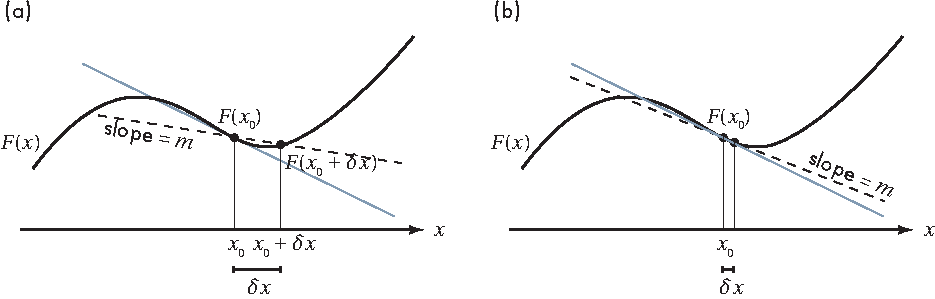
\includegraphics[]{math_primer/figures/dx.pdf}
  }
  \caption{Derivatives of functions.  The {\it slope} of a function at a point,
  $x_{0}$, can be approximated by taking the difference of the function
  evaluated at the point, $F(x_{0})$, and a nearby point, $F(x_0 + \delta\! x)$,
  divided by the distance, $\delta\! x$ between them.  The {\it derivative}
  represents the slope in the limit where $\delta\! x$ goes to 0.}
  \label{fig:dx}
\end{figure}

\subsubsection{Example}
Let us choose a simple function $F(x) = x^2$ as an example.  If we evaluate the
slope between $x_{0}$ and $x_{0} + \delta\! x$ we obtain
\begin{align*}
    m & \approx \frac{(x_0 + \delta\! x)^{2} - x_0^2}{\delta\! x} \\
      & \approx \frac{x_0^{2} + 2 x_0 \delta\! x + \delta\! x^{2} - x_0^2}{\delta\! x} \\
      & \approx \frac{2 x_0 \delta\! x + \delta\! x^2}{\delta\! x} \\
      & \approx 2 x_0 + \delta\! x.
\end{align*}
Applying the definition of the derivative (Equation~\ref{eq:derivative}),
\begin{equation*}
    \lim_{\delta\! x \to 0} (2 x_0 + \delta\! x) = 2 x_0.
\end{equation*}
Hence the slope (derivative), $m$, at the point of interest, $x_{0}$, is
\begin{equation*}
    m = \left. \dv{x^2}{x} \right|_{x = x_0} = 2 x_0.
\end{equation*}
For this function we can write the derivative at any point as
\begin{equation*}
    \dv{x^2}{x} = 2 x.
\end{equation*}

Derivatives can be a bit more difficult when the functions are not continuous or
smooth (a.k.a.\ not differentiable).  However, we often do wish to know the
derivative at these points in geophysics because they represent the boundaries
and interfaces---or discrete changes in behaviour with time---between
formations/rock types and their properties or their response to a physical
process.  In these cases, we often play games like taking the derivative from
each side of the boundary separately.  You have already seen this done as it was
performed on our circuit analogy with $\dd{u}\dd{t}$.  The function for the
changing transmitter current, $u(t)$, is continuous but not smooth.  For each
smooth segment of $u(t)$ the derivative is treated independent of the others
which resulted in three distinct behaviors within the conductive body.

\subsection{Chain Rule} \label{calc:chain}
There are few properties of derivatives more useful than the chain rule.  The
chain rule allows us to rewrite a complex function as a composite of simpler
functions.  Suppose we have a function $F(x)$ that we can write as a composite
of two or more functions, that is suppose we have another function $G(x)$ such
that $F(x) = F[G(x)]$.  Some examples of composite functions include,
\begin{align*}
    G(x) &= \sin x & F[G(x)] &= e^{G(x)} \\
    && &= e^{\sin x} ,
\end{align*}
\begin{align*}
    H(x) &= x^2 + z^2 & G[H(x)] &= H(x)^{1/2} & F\{G[H(x)]\} &= \frac{1}{G[H(x)]} \\
    && && &= \frac{1}{H(x)^{1/2}} \\
    && && &= \frac{1}{(x^2 + z^2)^{1/2}} .
\end{align*}

To find the derivative of such a function, we apply the chain rule,
\begin{equation*}
    \dv{}{x}F[G(x)] = \dv{F}{G}\dv{G}{x},
\end{equation*}
or more generally for a multiply compound function,
$f_0(f_1(f_2(\ldots f_{n-1}(f_n(x))\ldots))$,
\begin{equation}
    \dv{}{f_0(x)} = \dv{}{x}[f_0(f_1(f_2(\ldots f_{n-1}(f_n(x))\ldots))] =
    \dv{f_0}{f_1}\dv{f_1}{f_2}\cdots\dv{f_{n-1}}{f_n}\dv{f_n}{x} .
\end{equation}
What this allows us to do is take a complex function and break it into simpler
elements that can be easily differentiated (or at least make the derivatives
look like the forms given in a table of derivatives like the one located at the
end of this tutorial).

\subsubsection{Example}
Let's apply the chain rule to the second function above.  In order to find
$\dv{F}{x}$, we need the derivatives of $\dv{F}{G}$, $\dv{G}{H}$, and
$\dv{H}{x}$, all of which are general forms that we can find the table of
derivatives,
\begin{align*}
    1: && \dv{F}{G} &= \dv{}{G} \frac{1}{G} \\
    && &= -\frac{1}{G^2} \\
    2: && \dv{G}{H} &= \dv{}{H} H^{1/2} \\
    && &= \frac{1}{2 H^{1/2}} \\
    3: && \dv{H}{x} &= \dv{}{x} (x^2 + z^2) \\
    && &= 2 x.
\end{align*}
Now, we multiply each together and substitude each composite function to obtain
the derivative,
\begin{align*}
    \dv{F}{x} &= \dv{F}{G} \dv{G}{H} \dv{H}{x} \\
    &= \left(-\frac{1}{G^2}\right) \left(\frac{1}{2 H^{1/2}}\right) (2 x) \\
    &= \left(-\frac{1}{H^{\frac{1}{2} \cdot 2}}\right)
    \left(\frac{1}{2 (x^2 + z^2)^{1/2}}\right) 2 x \\
    &= \left(-\frac{1}{(x^2 + z^2)}\right)
    \left(\frac{1}{2 (x^2 + z^2)^{1/2}}\right) 2x,
\end{align*}
and finally simplifying,
\begin{equation*}
    \dv{F}{x} = - \frac{x}{(x^2 + z^2)^{3/2}} .
\end{equation*}

\subsection{Higher-order and partial derivatives}
There are also times when we wish to take higher order derivatives (e.g.\
acceleration is the second derivative of a distance function dependent upon
time).  In these cases the derivative operation is performed multiple times and
is mathematically represented by
\begin{equation}
    \dv[n]{}{x} F(x).
\end{equation}

A function may be dependent on multiple independent variables.  For example,
$F(x,y) = x^3y + y^2$ is a function of both $x$ and $y$.  We may take the
derivative of one or the other variables while treating the second constant.  We
call this operation the partial derivative where we use the symbol $\partial$ in
place of $d$.  For the above equation, the partial derivatives are
\begin{align*}
    \pdv{}{x}F(x,y) & = 3x^2y \\
    \pdv{}{y}F(x,y) & = x^3 + 2y.
\end{align*}
We can also take multiple derivatives in only one variable or both,
\begin{align*}
    \pdv[2]{}{x} F(x,y) & = 6xy \\
    \pdv[2]{}{y} F(x,y) & = 2 \\
    \frac{\partial^2}{\partial x \partial y} F(x,y) = 
    \frac{\partial^2}{\partial y \partial x} F(x,y) & = 3x^2. \\
\end{align*}
Note that when taking mixed derivatives, the result is independent of the order
in which the partials are taken.

\subsection{Table of Common Derivatives}
\begin{framed}
\noindent Derivatives of a few common functions (note $u = u(x)$, $v = v(x)$,
$a$ and $n$ are constants):
\begin{flalign*}
    &\dv{}{x}(a) = 0 &
    &\dv{}{x}(x) = 1 \\
    &\dv{}{x}(au) = a \dv{u}{x} &
    &\dv{}{x}(u + v) = \dv{u}{x} + \dv{v}{x} \\
    &\dv{}{x}(uv) = v\dv{u}{x} + u\dv{v}{x} &
    &\dv{}{x}\left(\frac{u}{v}\right) = v^{-2}\left(v\dv{u}{x} - u\dv{v}{x}\right) \\
    &\dv{}{x}u(v) = \dv{u}{v}\dv{v}{x} &
    &\dv{y}{x} = \left( \dv{x}{y} \right)^{-1} \\
    &\dv{}{x}(u^n) = n u^{n-1} \dv{u}{x} &
    &\dv{}{x}\left(\frac{1}{u^n}\right) = -\frac{n}{u^{n + 1}} \dv{u}{x} \\
    &\dv{}{x}(e^u) = e^u \dv{u}{x} & 
    &\dv{}{x}(\log u) = \frac{1}{u} \dv{u}{x},\; u > 0 \\
    &\dv{}{x}(\sin u) = \cos u \dv{u}{x} &
    &\dv{}{x}(\cos u) = -\sin u \dv{u}{x}
\end{flalign*}
\end{framed}



% ---------------------------------------
\section{Integrals} \label{apx:integral}
\subsection{Definition}
Integrals (anti-derivatives) perform the inverse operation of a derivative.  Its
technical definition is
\begin{equation*}
    \dv{}{x} \int_{0}^{x} f(t) \dd{t} \equiv f(x),
\end{equation*}
and while this is accurate and establishes that integration is in fact the
anti-derivative, it is basically useless for understanding how it works.  So
lets approach the integral from another way.

If a derivative represents the differences of small steps, integrals represent
the sum of small steps.  Since we divided before by $\delta x$, this time we
will do the opposite and multiply, suggesting that the integral represents an
area under a curve (Figure~\ref{fig:ix}).
\begin{figure}[hbt]
  \centerline{
    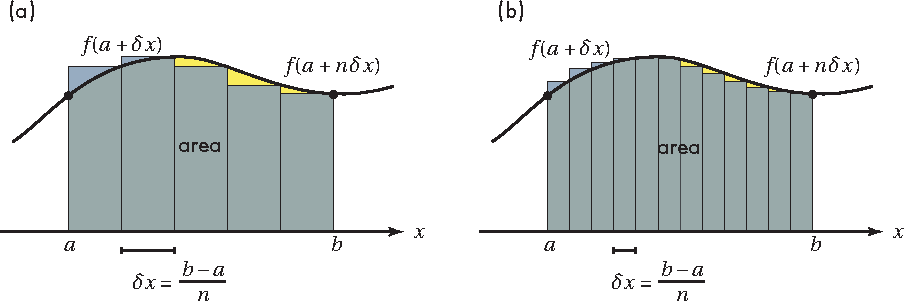
\includegraphics[]{math_primer/figures/ix.pdf}
  }
  \caption{Integrals of functions.  The {\it area} under a function between two
  points, $a$ and $b$, can be approximated by the sum of $n$ small columns with
  height $f(a + i \delta\!  x)$ and width $\delta\! x = (b - a)/n$.  The {\it
  integral} represents the area in the limit where $n$ goes to infinity.}
  \label{fig:ix}
\end{figure}

Consider a function $f(x)$ finite on the interval $[a, b]$ ($a \leq x \leq b$).
A simple method for approximating the area is performed by dividing the curve
into several rectangular elements and summing the individual area of each.  For
$n$ steps in $x$, the width of the step is $\delta\! x = (b - a)/n$.  To find
the area of each element, we multiply the step size, $\delta\! x$ by the value
of the function within the $i$-th step, $f(\bar{x}_i)$.  It does not matter
where we choose the value of the function so long as it is between the interval
bounds, $x_i$ to $x_{i+1}$, because as the interval width appoaches zero the
value of the fuction on each side of the interval approach the same value.
Summing each element gives an estimate of the total area, 
\begin{equation*}
    A \approx \sum_{i = 1}^{n} f(\bar{x}_{i}) \delta x.
\end{equation*}
A more useful definition for the purposes of determining an integral employs the
limit as $n$ goes to infinity ($\infty$),
\begin{equation*}
    \int_{a}^{b} f(x) \dd{x} \equiv \lim_{n \to \infty} \sum_{i = 1}^{n}
        f(\bar{x_{i}}) \frac{b - a}{n}.
\end{equation*}

There are a few integrals that are quite common and tend to show up frequently
in derivations.  The solutions to these integrals are commonly listed in `{Tables
of Integrals}' which you can easily find using a web search under the same name.
You will find thousands all of which are 95\% the same.  Mathworld has a pretty
good one, as does Wikipedia.  I use a copy of the Standard Mathematical Tables
and Formula from the CRC Press.

\subsection{Example}
Consider the result from our derivative example, $f(x) = 2 x$, we will integrate
this result to (1) illustrate how an integral is determined by a sum of
infinitely man small areas
and (2) show that the integral of a derivative has the same form of our original
function.

As we discussed above, the area of a column is given by the height,
found by evaluating our function some point within the bounds of th column,
multiplied by the width of the column, i.e.,
\begin{align*}
    A_i &\approx f(\bar{x}_i) \delta\! x \\
    &\approx 2 \bar{x}_i \delta\! x .
\end{align*}
The total area of all the columns is then
\begin{align*}
    A &\approx A_1 + A_2 + A_3 \ldots A_n \\
    &\approx \sum_{i=1}^n A_i .
\end{align*}
Therefore, including the individual areas in terms of our function as above, the
sum becomes
\begin{equation*}
    A \approx \sum_{i = 1}^{n} 2 \bar{x}_i \delta\! x .
\end{equation*}
If we choose $\bar{x}_i$ at a convenient location, say at the lower bound to the
column width.  The $x$ coordintes that the function is evaluated at are $a$, $a
+ \delta\! x$, $a + 2\delta\! x$ and so on.  This allows us to write the area
as,
\begin{align*}
      A &\approx \left[ 2 (a + \delta\! x) + 2 (a + 2 \delta\! x) 
        + \ldots + 2 (a + n \delta\! x) \right] \delta\! x \\
      &\approx \sum_{i = 1}^{n} (2 a \delta\! x + 2 i \delta\! x^2).
\end{align*}
The first sum is trivial, the second requires knowing that $\sum_{i=1}^{n} i = n
(n + 1)/2$.  Thus the summation becomes
\begin{equation*}
    A \approx 2 a n \delta\! x + n (n + 1) \delta\! x^2.
\end{equation*}
Now inputting the definition of $\delta\! x$, we have
\begin{align*}
    A & \approx 2 a n \frac{b - a}{n} + n (n + 1) \frac{(b - a)^2}{n^2} \\
      & \approx 2 a (b - a) + \left( 1 + \frac{1}{n} \right) (b - a)^2 \\
      & \approx 2 a b - 2 a^2 + (b - a)^2 + \frac{(b - a)^2}{n} \\
      & \approx 2 a b - 2 a^2 + b^2 - 2 a b + a^2 + \frac{(b - a)^2}{n} \\
      & \approx b^2 - a^2 + \frac{1}{n}(b - a)^2 \\
\end{align*}
Now we can introduce the limit again only it as the number of intervals goes to
infinity,
\begin{equation*}
    \lim_{n \to \infty} b^2 - a^2 + \frac{1}{n}(b - a)^2 = b^2 - a^2.
\end{equation*}
Therefore, the integral from $a$ to $b$ of $2 x$ is
\begin{equation*}
    \int_{a}^{b} 2 x \dd{x} = \left. x^2 \right|_{a}^{b} = b^2 - a^2.
\end{equation*}

We have now shown that the integral in this case is indeed the anti-derivative.
Another important implication is that the integral depends only upon the bounds
of integration, $a$ and $b$, which is true in general and not just for this
example.

\subsection{Indefinite integrals}
The above result is called the definite integral because it has defined limits
of integration, but there are many times we wish to have arbitrary integration
limits.  When the limits are arbitrary we call this the indefinite integral, and
it is written as
\begin{equation}
    \int f(x) = F(x) + C.
\end{equation}
For our previously worked example, the indefinite integral is
\begin{equation*}
    \int 2 x \dd{x} = x^2 + C,
\end{equation*}
where $C$ is an arbitrary constant.  The constant arises from the fact that a
derivative of a constant is 0, so the general anti-derivative must allow for
the possibility of a constant that vanished under the derivative operation.

\subsubsection{Example}
Let us take the function,
\begin{equation*}
    f(x) = x e^{-x^2} .
\end{equation*}
To take the integral,
\begin{equation*}
    \int f(x) \dd{x} = \int x e^{-x^2} \dd{x} ,
\end{equation*}
we need to put the integral into a form that we can find in an integral table.
Looking at the table of integrals, the closest integral we can find is
\begin{equation*}
    \int e^u \dd{u} = e^u \dd{u} .
\end{equation*}
We will also need the integral property,
\begin{equation}
    \int u(v) \dd{x} = \int u \left(\dv{v}{x}\right)^{-1} \dd{v} ,
\end{equation}
to rewrite our function into the simplified form we desire.  So let us define a
function
\begin{align*}
    v(x) &= -x^2 \\
    \dv{v}{x} &= -2x \\
    - \frac{1}{2x} \dd{v} &= \dd{x} .
\end{align*}
Substituting in the $v(x)$ and the expression for $\dd{x}$, we find 
\begin{equation*}
    \int x e^{-x^2} \dd{x} = \int x e^{v} \left( - \frac{1}{2x} \dd{v} \right) .
\end{equation*}
Simplifying and bringing the constants outside the integral,
\begin{equation*}
    \int x e^{-x^2} \dd{x} = - \frac{1}{2} \int e^{v} \dd{v} \\
\end{equation*}
Since this now looks like our elementary form, all we need to do is complete the
integration and back subsitute the $v(x)$.
\begin{align*}
    \int x e^{-x^2} \dd{x} &= - \frac{1}{2} e^{v} \\
    &= - \frac{1}{2} e^{-x^2} .
\end{align*}


\subsection{Multiple integrals}
Again there are times where we wish to integrate multiply say for area
(2-dimensional) or volume (3-dimensional) calculations.  The area can be written
\begin{equation}
    \iint f(x,y) \dd{x} \dd{y} = \int_{A} f(x,y) \cdot \dd{\vb{a}},
\end{equation}
where $\dd{\vb{a}}$ implies area infintesimals and for volume,
\begin{equation}
    \iiint f(x,y,z) \dd{x} \dd{y} \dd{z} = \int_{V} f(x,y,z) \cdot \dd{\vb{v}},
\end{equation}
where $\dd{\vb{v}}$ implies volume infintesimals.  Note that the order in which
we perform the integrations is irrelevant to the solution (although in reality,
our choice of order may make it easier to derive).

\begin{framed}
    {\bf Aside:} In reality, the derivative or integral of a function may be
    very complex, or we do not know {\it a priori} (beforehand) the exact nature
    of the originating function.  In these cases, we use numerical techniques
    not terribly dissimilar from the original algebraic starting points, i.e.\
    with differences and sums of small intervals.
\end{framed}

A table of integrals is often far handier than a table of derivatives since the
chain rule can be successively applied to make each step closer to an elementary
form.  To give you an indication how much more challenging integrals can be, the
table of derivatives in the {\it Standard Mathematical Tables and Formulae}
covers common derivatives in two pages and provides 44 pages of integrals.  But
never fear, we will only use a few and if use one not in the table, I will
provide you with the relevant general forms if you need them to complete
problems.

\subsection{Table of Common Integrals}
\begin{framed}
\noindent Integrals of a few common functions (note $u = u(x)$, $v = v(x)$,
$a$ and $n$ are constants and $C$ is an arbitrary constant due to integration):
\begin{flalign*}
    &\int a \dd{x} = a x + C &
    &\int x \dd{x} = \frac{1}{2}x^2 + C \\
    &\int au \dd{x} = a \int u \dd{x} &
    &\int (u + v) \dd{x}  = \int u \dd{x} + \int v \dd{x} \\
    &\int u \dd{v} = uv - \int v \dd{u} &
    &\int u(v) \dd{x} = \int u(v) \left( \dv{v}{x} \right)^{-1} \dd{v} \\
    &\int u^n \dd{u} = \frac{1}{n+1} u^{n+1} + C, \; n \neq -1 &
    &\int \frac{1}{u} \dd{u} = \log u + C \\
    &\int e^{u} \dd{u} = e^{u} + C &
    &\int \log u \dd{u} = u \log u - u \\
    &\int \sin u \dd{u} = -\cos u + C &
    &\int \cos u \dd{u} = \sin u + C 
\end{flalign*}
\end{framed}


\nocite{Zwillinger1996}
\bibliographystyle{elsarticle-harv}
\bibliography{ref}
